\section{Background to the Research}
\vspace{12pt}


Sri Lankan government is still using lots of manual processes for identity verification of people. 
People have to keep providing their legal documents in order to work with the authority. There are 
several basic legal documents like “Birth Certificate”, “National Identity Card”, “Driving License”, 
“Passport”  for a person in Sri Lanka. And also have other qualification certificates like “ University 
Transcript”, “School Leaving Certificate”, “Character Certificate” and more. The current process is, 
people have to provide their information in a legal manner and claim their assertions. When they need 
to interact with the authority, they should provide the same information or assertions over again. 
The problem in this context is people provide their very same information or assertions on different 
authority sectors and organizations. This is a major problem when considering the government sectors. 
Since there are millions of people in a country, a government needs a provable claim to identify and 
verify people. 

\vspace{12pt}


Official evidence of identity is basic to a person's capacity to implement their privileges and secure 
access to a wide scope of essential administrations, for example, medicinal services, training, portable 
availability, social assurances, and budgetary administrations. Sri Lanka has essential and practical 
personality frameworks that are very much evolved and hearty. Responsibility for National Identity Card 
(NIC) is high, revealed at 95 percent for men and 90 percent for ladies, with just little pockets of Sri 
Lankan culture more averse to claim a NIC. Birth Certificates and National Identity Cards are major 
identities for verification in Sri Lanka. However, the Birth certificate is a mandatory document for 
claiming the National Identity Card. But most of the time people need to present both NIC and Birth 
certificate. When people need to apply for a Driving license or a university enrollment, again they 
need to present their birth certificate. This is where the duplication of identity verification happens.
 Because of this duplication process, people have to submit their verification documents continuously. 
 And it is more costly and time-wasting criteria. The Sri Lankan government produces more than 300,000 
 birth certificates per year. The birth certificate is the most fundamental identity for identity verification 
 in Sri Lanka.

 \begin{figure}[H]
    \centering
    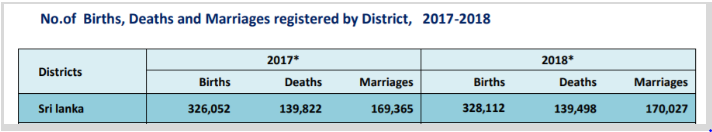
\includegraphics[scale=1]{Capture.png}
    \caption{Sri Lankan Registration certificates}
    \label{fig:threshold}
  \end{figure}

  Birth certificate issued by the Sri Lankan government when birth and every person has it with them. 
  For instance, Pasindu is a civilian in Sri Lanka and has to provide her identity for school applying. 
  Then Pasindu needs to enter a state university and again needs to provide the birth certificate. 
  When Pasindu wants to apply for a driving license, again he needs to present his birth certificate 
  as her identity document. As a solution to this problem, the government can consider a centralized 
  system[1] with a centralized database[2] for identity verification.
  
  \begin{figure}[H]
    \centering
    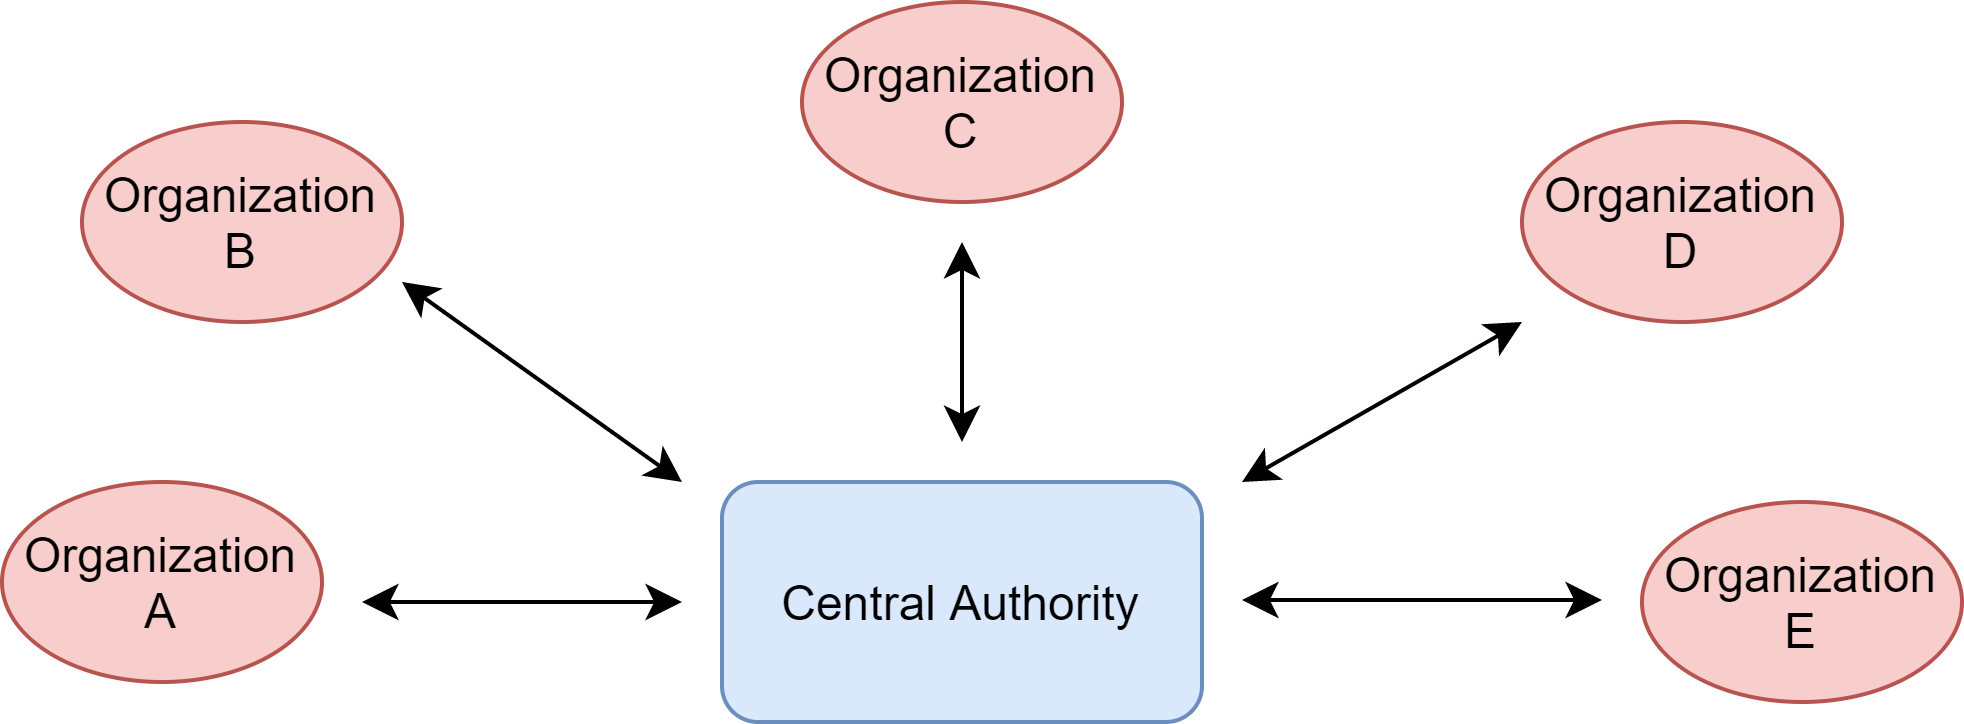
\includegraphics[scale=0.8]{1.png}
    \caption{centralized database}
    \label{fig:threshold}
  \end{figure}

  Centralized systems are systems that use client/server architecture where one or more client nodes 
  are directly connected to a central server. This is the most commonly used type of system in many 
  organizations where the client sends a request to a company server and receives the response. 
  In this centralized system, the government can record the identities of civilians and provide 
  an application program interface (API) for organizations and government sectors that need to 
  verify the identities. Organizations and the government should have a mutual trust for verifying 
  identities. For instance, Alice can verify her claim which could be the birth certificate or any 
  verifiable document with the authority and get an assertion for her claim document. Then Alice 
  can use this assertion when she wants to apply for a driving license. But this centralized 
  system has some limitations and problems.

  \subsection{Limitations}

  \begin{itemize}
    \item It cannot scale up vertically after a certain limit. After this limit, even if it increases 
    the hardware and software capabilities of the server node, the performance will not increase 
    appreciably leading to a cost/benefit ratio < 1.
    \item Bottlenecks can appear when the traffic spikes – as the server can only have a finite number
     of open ports to which can listen to connections from client nodes. So, when high traffic occurs
      like a shopping sale, the server can essentially suffer a Denial-of-Service attack or Distributed
       Denial-of-Service attack.
      
  \end{itemize}

  \subsection{Problems}

  \begin{itemize}
    \item Highly dependent on the network connectivity – System can fail if the nodes lose connectivity as there is only one central node.
    \item No graceful degradation of the system – abrupt failure of the entire system
    \item Less possibility of data backup. If the server node fails and there is no backup, system lose the data straight away
    \item Difficult server maintenance – There is only one server node and due to availability reasons, it is inefficient and unprofessional to take the server down for maintenance. So, updates have to be done on-the-fly(hot updates) which is difficult and the system could break.
    \item Only the government can authorize users.
  \end{itemize}

  To overcome the above limitations and problems, the authority can think of a decentralized solution[3]. 
  In this decentralized system, the government can distribute the centralized database throughout the 
  organizations that are already trusted by the government.

  \begin{figure}[H]
    \centering
    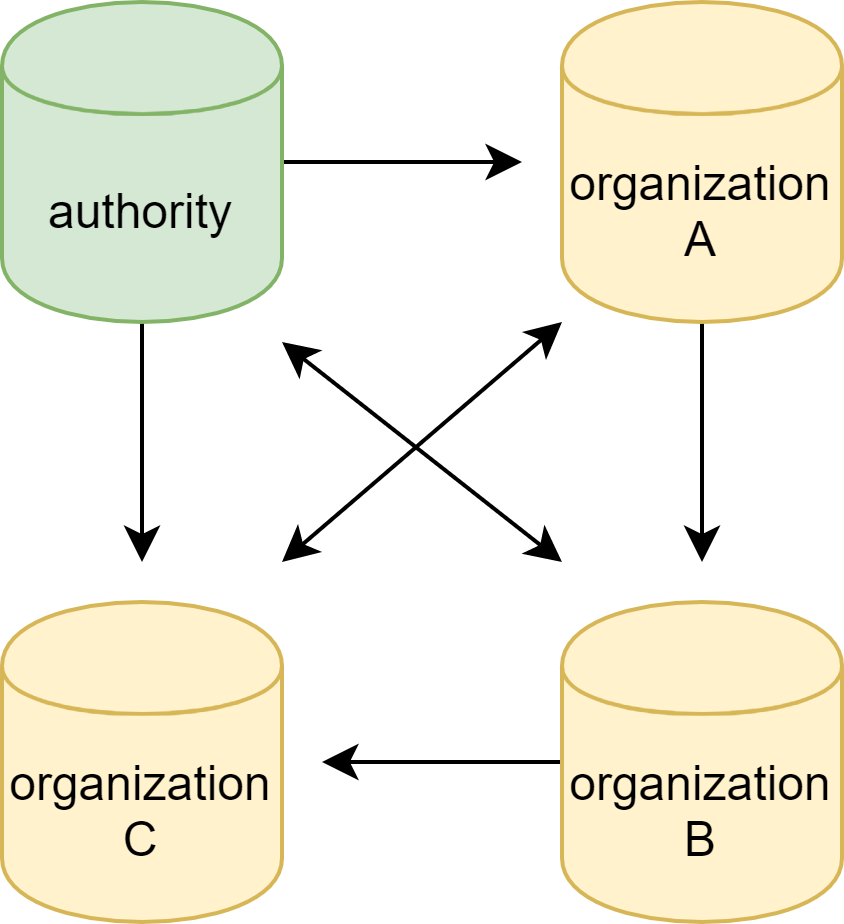
\includegraphics[scale=1]{2.png}
    \caption{decentralized database}
    \label{fig:threshold}
  \end{figure}

  The authority can provide privileges for organizations to verify assertions. But still, the 
  government has the ability to provide privileges and there is no transparency. There are some 
  problems in a system like above to archive the following properties.

  \begin{enumerate}
      \item Existence - Users must have an independent existence.
      \item Control -  Users must control their identities.
      \item Access - Users must have access to their own data.
      \item Transparency - Systems and algorithms must be transparent.
      \item Persistence - Identities must be long-lived.
      \item Portability - Information and services about identity must be transportable
      \item Interoperability - Identities should be as widely usable as possible.
      \item Consent - Users must agree to the use of their identities.
      \item Minimization - Disclosure of claims must be minimized.
      \item Protection - The rights of users must be protected.
  \end{enumerate}

  Authorities cannot archive the above properties using a decentralized database solution. 
  The only possible solution to archive those targets is using blockchain[4] architecture. 
  The blockchain network has no central authority and it is the very definition of a 
  democratized system. Since it is a shared and immutable ledger, the information in it is 
  open for anyone and everyone to see. Hence, anything that is built on the blockchain is 
  by its very nature transparent and everyone involved is accountable for their actions. 
  And it is possible to implement the above properties on top of a blockchain model rather 
  than a decentralized database.


  




\clearpage



